\let\negmedspace\undefined
\let\negthickspace\undefined
\documentclass[journal]{IEEEtran}
\usepackage[a5paper, margin=10mm, onecolumn]{geometry}
\usepackage{lmodern} % Ensure lmodern is loaded for pdflatex
\usepackage{tfrupee} % Include tfrupee package

\setlength{\headheight}{1cm} % Set the height of the header box
\setlength{\headsep}{0mm}     % Set the distance between the header box and the top of the text

\usepackage{gvv-book}
\usepackage{gvv}
\usepackage{cite}
\usepackage{amsmath,amssymb,amsfonts,amsthm}
\usepackage{algorithmic}
\usepackage{graphicx}
\usepackage{textcomp}
\usepackage{xcolor}
\usepackage{txfonts}
\usepackage{listings}
\usepackage{enumitem}
\usepackage{mathtools}
\usepackage{gensymb}
\usepackage{comment}
\usepackage[breaklinks=true]{hyperref}
\usepackage{tkz-euclide} 
\usepackage{listings}
\usepackage{gvv}                                        
\def\inputGnumericTable{}                                 
\usepackage[latin1]{inputenc}                                
\usepackage{color}                                            
\usepackage{array}                                            
\usepackage{longtable}                                       
\usepackage{calc}                                             
\usepackage{multirow}                                         
\usepackage{hhline}                                           
\usepackage{ifthen}                                           
\usepackage{lscape}
\begin{document}

\bibliographystyle{IEEEtran}
\vspace{3cm}

\title{12.6.6.10}
\author{EE24BTECH11003 - Akshara Sarma Chennubhatla}
% \maketitle
% \newpage
% \bigskip
{\let\newpage\relax\maketitle}
\textbf{Question:}
The sum of the perimeter of a circle and square is $k$, where $k$ is some constant. Prove that the sum of their areas is least when the side of square is double the radius of the circle.

\solution\\

The method used to solve this question is the gradient descent.\\
Taking the radius of the circle as $r$ and the side of the square as $a$, through given information,
\begin{align}
	2\pi r + 4a = k\\
\end{align}
We need to minimize
\begin{align}
	\pi r^2 + a^2\\
\end{align}
and prove that at the minimum sum of areas point, $a = 2r$.\\
Substituting $\brak{1}$ in $\brak{2}$,
\begin{align}
	A\brak{r} &= \pi r^2 + \brak{\frac{k - 2\pi r}{4}}^2\\
	A\brak{r} &= \brak{\frac{\pi^2}{4} + \pi}r^2 - \frac{\pi k}{4}r + \frac{k^2}{16}
\end{align}
Applying Gradient Descent to this function,
\begin{align}
	r_{n+1} &= r_n - \mu A^\prime\brak{r_n}\\
	A^\prime\brak{x} &= 2\brak{\frac{\pi^2}{4} + \pi}r - \frac{\pi k}{4}\\
	r_{n+1} &= r_n\brak{1 - 2\mu\brak{\frac{\pi^2}{4} + \pi}} + \frac{\mu\pi k}{4}
\end{align}
Applying unilateral Z-transform,
\begin{align}
	zR\brak{z} - zr_0 &= R\brak{z}\brak{1 - 2\mu\brak{\frac{\pi^2}{4} + \pi}} + \frac{\mu\pi k}{4} \frac{1}{1 - z^{-1}}\\
	R\brak{z} &= \frac{zr_0}{z - \brak{1 - 2\mu\brak{\frac{\pi^2}{4} + \pi}}} + \frac{\mu\pi k}{4} \frac{1}{1 - z^{-1}}\\
	R\brak{z} &= \frac{zr_0}{z - \brak{1 - 2\mu\brak{\frac{\pi^2}{4} + \pi}}} + \frac{k}{10 \pi \brak{z - 1}} - \frac{k \brak{1 - 2\mu\brak{\frac{\pi^2}{4} + \pi}}}{10 \pi \brak{z - \brak{1 - 2\mu\brak{\frac{\pi^2}{4} + \pi}}}}\\
	R\brak{z} &= \frac{r_0}{1 - z^{-1}\brak{1 - 2\mu\brak{\frac{\pi^2}{4} + \pi}}} + \frac{kz^{-1}}{10 \pi \brak{1 - z^{-1}}} - \frac{z^{-1}k \brak{1 - 2\mu\brak{\frac{\pi^2}{4} + \pi}}}{10 \pi \brak{1 - z^{-1}\brak{1 - 2\mu\brak{\frac{\pi^2}{4} + \pi}}}}\\
\end{align}
From this equation, the ROC is,
\begin{align}
	\abs{z} > max\brak{\abs{1 - 2\mu\brak{\brak{\frac{\pi^2}{4} + \pi}}},1}\\
	\implies \abs{z} >
	\begin{cases}
		1 &, \mu > 0\\
		1 - 2\mu\brak{\brak{\frac{\pi^2}{4} + \pi}} &, \mu < 0\\
	\end{cases}
\end{align}
Assuming $\mu$ satisfies the above condition,
\begin{align}
	\lim_{n\to\infty}\norm{r_{n+1} - r_n} &= 0\\
	\lim_{n\to\infty}\norm{\frac{\mu k\pi}{4} - r_n2\mu\brak{\frac{\pi^2}{4} + \pi}} &= 0\\
	\implies \lim_{n\to\infty}\norm{r_n} &= \frac{k}{8\brak{\frac{\pi}{4} + 1}}
\end{align}
But, we know that,
\begin{align}
	2\pi r_n + 4a_n &= k\\
	2\pi \brak{\frac{k}{2\brak{\pi + 4}}} + 4a_n &= k\\
	\implies a_n &= \frac{k}{\pi + 4}\\
	\implies a_n &= 2r_n
\end{align}
Thus, it is proved that at minimum condition, the length of the side of the square is double the radius of the circle.

Below is the plot for the area vs radius graph with initial conditions as follows,
\begin{align}
	r_0 &= -10\\
	\mu &= 0.001\\
	\text{tolerance of convergence} &= 10^{-6}\\
	k &= 10\pi\\
\end{align}
The point of minima we get is,
\begin{align}
	x_{min} = 2.199416...
\end{align}

\begin{figure}[h!]
	\centering
	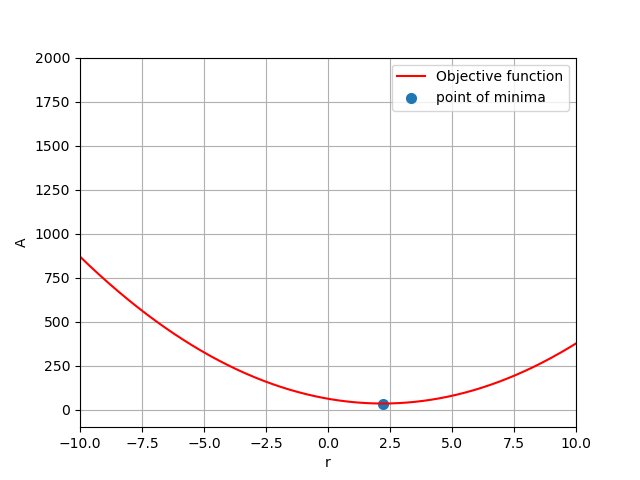
\includegraphics[width=1\columnwidth]{figs/simulated.png}
	\caption{Plot of the area vs radius}
	\label{stemplot}
\end{figure}

\end{document}
